\chapter{RDF Graph Builder}
\label{chp:rdf-builder}

A fundamental part for providing \acl{LOD} on the Web is to build the \ac{RDF} Graph from the available data. The main obstacle in this project is the fact that different municipalities and public organizations may model the data in different ways, thus making the process of mapping the data into an \ac{RDF} Graph in accordance with the \ac{OntoIM} and OntoPiA ontologies difficult. The main idea, as shown in Figure \ref{fig:rdf-builder-architecture}, is to collect and process data from different sources: the city's CKAN portal, offline files, and Open Data published by state and regional agencies. Thus, two libraries were made in Python to simplify graph creation through object-oriented programming by converting ontology classes into Python classes, and related properties into attributes. This makes data entry from the various sources easier and code reading more understandable. Both the Python libraries and the \ac{RDF} Graph builder also make use of well-known libraries such as \verb#pandas# and \verb#rdflib# for data manipulation and reading, and graph creation and serialization. Finally, the sources of the various resources and other configurations are all defined in a single \verb#conf.ini# file to allow for better control and easier editing. An example of this file is shown in Code \ref{code:config-ini}.

\begin{lstlisting}[caption={Example of a config.ini file that defines sources for some semantic areas.},label=code:config-ini]
[ANNCSU]
streets = anncsu/streets.csv
civics = anncsu/civics.csv
census_sections = anncsu/census_sections.kml
post_code = 37060

[ORGANIZATIONS]
organizations = organizations/organizations.csv

[WASTE]
waste_production = waste/waste_production.csv
\end{lstlisting}

Resources will be grouped into datasets defined as \verb#dcat:Dataset#, and, for the specific case of the Comune di Sona, will be identified by \acp{URL} formatted as follows:

\begin{verbatim}
  https://w3id.org/sona/data/{dataset_id}/.../{resource_id}
\end{verbatim}

The \verb#dataset_id# is the identifier of the dataset (e.g. \textit{schools}, \textit{demographic-observations}, \etc), while the \verb#resource_id# is the identifier of the resource, which is generated following different formats depending on the resource. Some supporting resources (e.g., geographic locations or time intervals) may also be located in additional paths that define the resource type (e.g. \textit{geo} or \textit{ti}).

\begin{figure}[!ht]
  \centering
  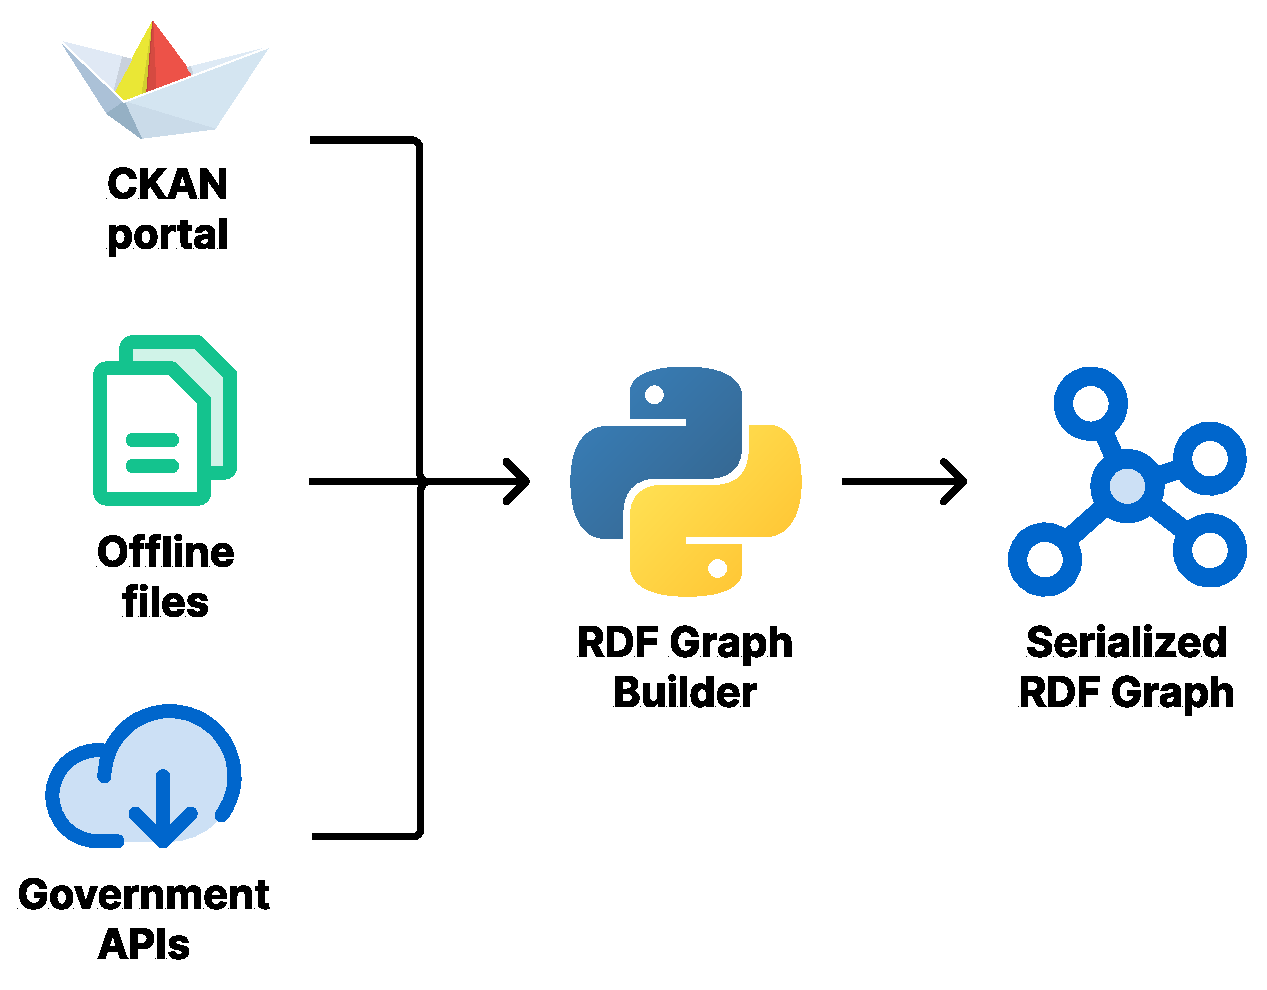
\includegraphics[width=0.6\columnwidth]{images/ontoim/rdf-graph-builder}
  \caption{\ac{RDF} Graph Builder architecture.}
  \label{fig:rdf-builder-architecture}
\end{figure}

Section \ref{sec:onto-py} will describe the Python libraries developed to facilitate the creation of the \ac{RDF} Graph, while Section \ref{sec:workflows-sas} will present some examples of data mapping for different data and semantic areas.

\subimport{}{01_onto_py}%
\subimport{}{02_workflow_sas}%